\vspace{-0.3cm}
\section{Design}
\vspace{-0.1cm}
%
This section describes the MX-based mixed-precision quantization scheme and the \sysname accelerator architecture. 
%
%In this section, we discuss low-precision MX quantization design of \sysname.
% Our approach leverages MX, addressing the challenges posed by activation outliers while further optimizing efficiency.

\vspace{-0.35cm}
\subsection{Magnitude-based Mixed-Precision MX Quantization}
%
\niparagraph{Mixed-precision quantization for linear layers.}
%
Figure~\ref{fig:observation} reports that large-magnitude values concentrate in specific channels, while outliers consistently appear in the same ones regardless of the prompt~\cite{qdit}. 
% 
Given the observation, we propose a mixed-precision quantization scheme for linear layers, utilizing a channel-wise reordering technique as shown in Figure~\ref{fig:linear}.
%
\sysname first reorders channels according to their average magnitude, clustering outliers and inliers together to prevent the inlier truncation caused by outliers within the same group.
%
It then reorders weight channels following the same order as the activation channels.
%
After reordering, \sysname quantizes activation channels with large-magnitude values using high precision (MX9), while applying low precision (MX6) to channels with small-magnitude values and weight matrices.
%
The proportion of activation channels quantized with MX9 is controlled by a hyperparameter, $p_1$, whose its determination mechanism will be discussed in Section~\ref{subsec:hyperparam-selection}. 
%
% linear layer 에서의 observation 에 따르면, activation matrix 에서의 outlier 는 어떤 input prompt 든지, 어떤 token 인지와 상관없이 outlier 가 있는 channel 은 동일함.
% 이에 우리는 channel-wise reordering 을 통해 outlier 는 outlier 끼리, inlier 는 inlier 끼리 group 되게 해 outlier에 의한 inlier 의 truncation 을 막음. 
% 또한, channel reordering 후 outlier 가 있는 channel 은 high precision 으로 quantize 하여, outlier 값을 보존함. 
% high precision 으로 양자화할 channel 개수의 비율을 p_1 이라는 hyperparameter 로 설정함. 
% p_1 값을 어떻게 결정하는지에 대해서는 B. offline hyperparemeter selection 에서 다룰 것. 

\begin{figure}[t]
\centering
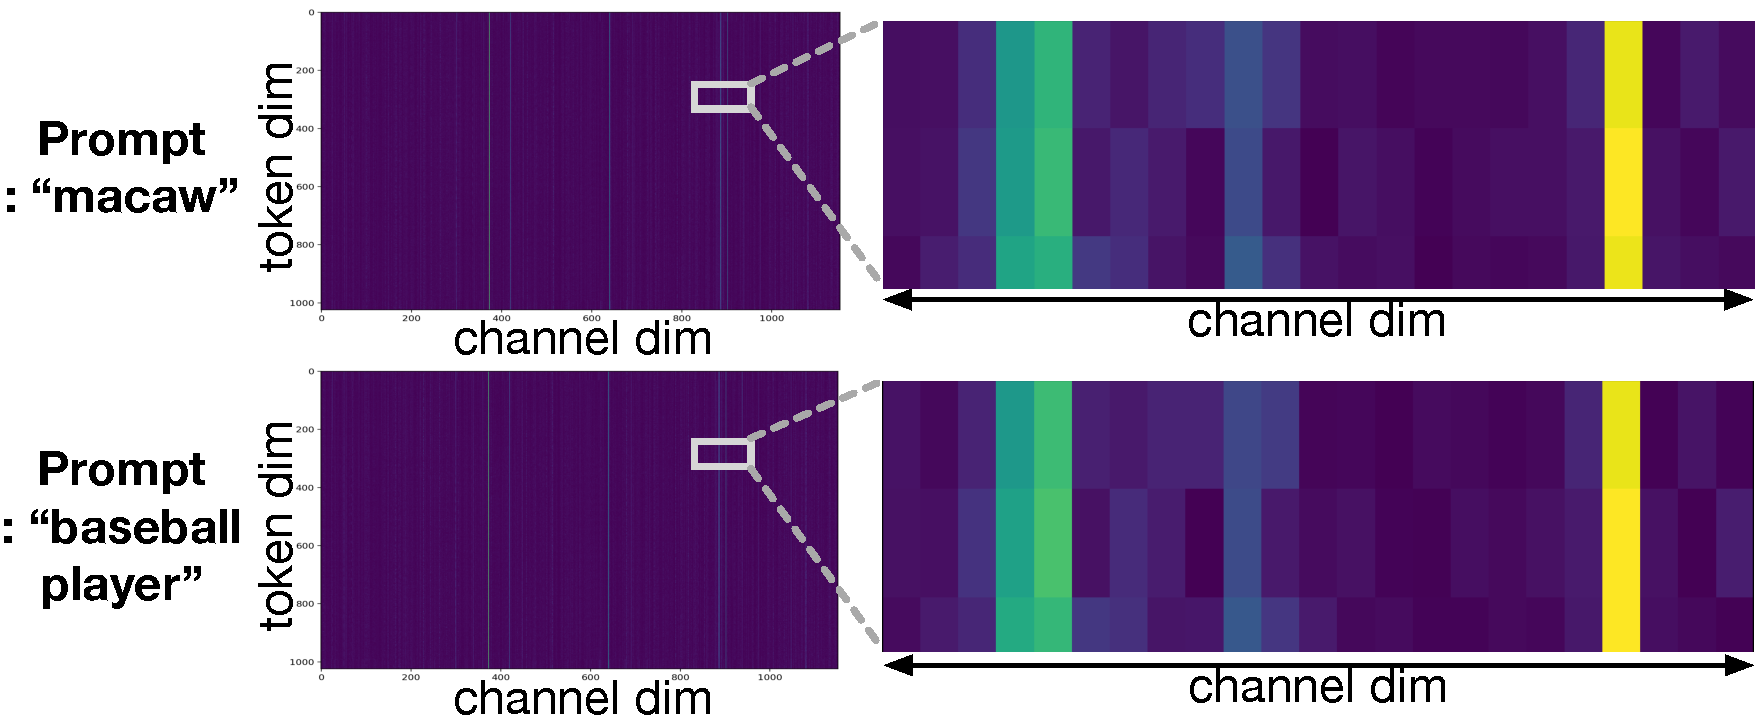
\includegraphics[width=0.8\linewidth]{fig/observation.pdf}
\caption{Observation of linear layer activation's value magnitude in DiT-XL-512. The colors mean same with Fig.~\ref{fig:distribution}.}
\label{fig:observation}
\end{figure}

% Figure
\begin{figure}[t]
\centering
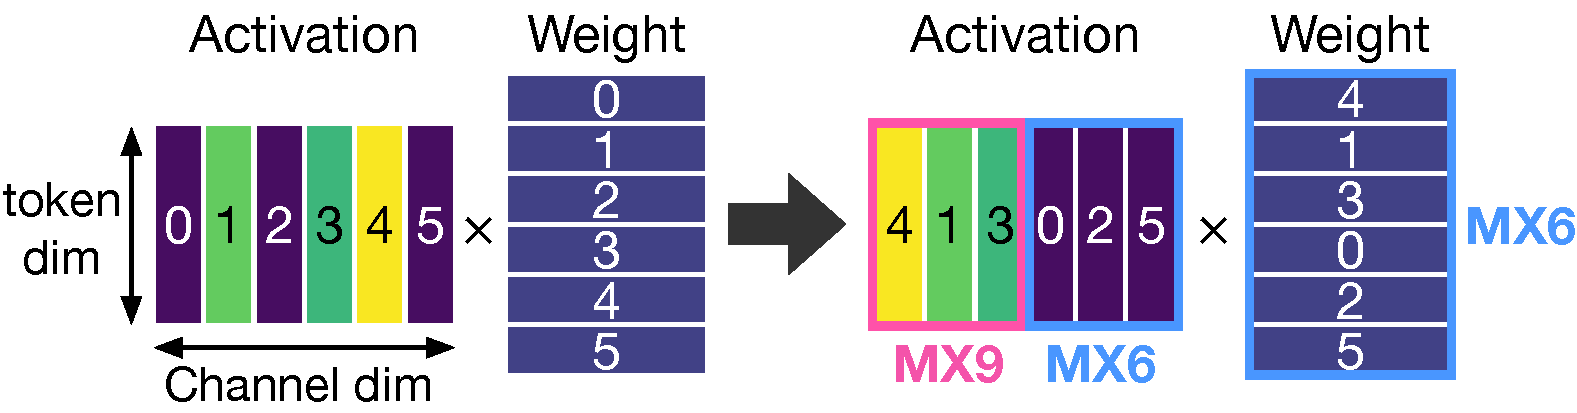
\includegraphics[width=0.9\linewidth]{fig/linear.pdf}
\caption{Channel-wise reordering and mixed precision in linear layer. The colors mean same with Fig.~\ref{fig:distribution}.}
\label{fig:linear}
\end{figure}

%
\niparagraph{Mixed-precision quantization for attention layers.}
%
The attention layer, performing activation-activation multiplication, requires a different approach.
%
Figure~\ref{fig:attention} delineates the scheme.
%
In multi-head attention, each head independently performs the $Q\times K^T$ and $Softmax\times V$ operations. 
%
Unlike the linear layer, where outliers are present at the channel level, the attention layer exhibits them at the head level. 
%
Analyzing 1,000 COCO prompts, we observed that as in channels in the linear layer, large-magnitude heads remain consistent across various inputs, allowing offline identification.
% 
In our head-wise mixed-precision design, heads with large average magnitudes are quantized with MX9, while those with small magnitudes use MX6. 
%
As with the linear layer, the proportion of heads quantized with MX9 is controlled by a hyperparameter, $p_2$.
% 
% \begin{align}
% p_2 &= \frac{\#\text{heads\_for\_MX9}}{\#\text{heads}} \times 100 (\%)
% \end{align}
% 
% Attention layer 는 activation-activation multiplication 을 하는 layer 이기 때문에 linear layer 와는 다른 방식이 필요하다. 
% multi-head attention 에서의 Q*K^T 연산과 S*V 연산은 각 head 별로 이루어짐.
% channel 단위로 outlier 가 존재했던 linear layer 와는 다르게, attention layer 에서는 head 단위로 outlier 가 존재함. 
% 따라서, average magnitude 가 큰 head 들은 high precision 으로 quantize 하고, 그렇지 않은 head 들은 low precision 으로 quantize 하는 방식을 사용함.
% high precision 을 사용할 head 의 비율을 p_2 라는 hyperparamter 로 설정하였음.

% Figure
\begin{figure}[t]
\centering
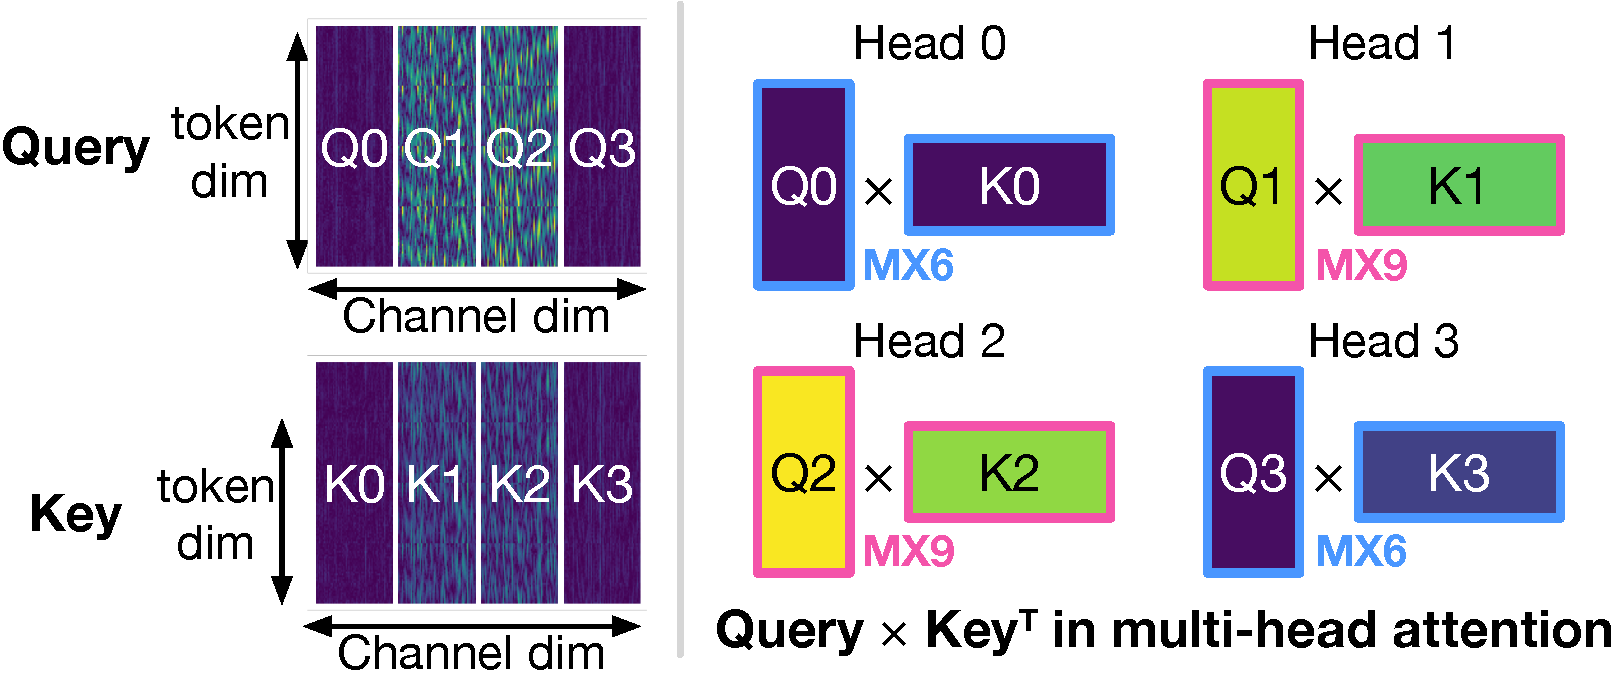
\includegraphics[width=0.9\linewidth]{fig/attention.pdf}
\caption{Head-wise mixed precision in multi-head attention layer. The colors mean same with Fig.~\ref{fig:distribution}.}
\label{fig:attention}
\end{figure}

\vspace{-0.3cm}
\subsection{Offline Hyperparameter Determination} 
\vspace{-0.1cm}
\label{subsec:hyperparam-selection}
%
\niparagraph{Importance of the hyperparameters.}
%
Figure~\ref{fig:tradeoff} shows the quality-latency tradeoff according to the hyperparameter $p_1$ and $p_2$.
%
As the $p_1$ and $p_2$ increase, a larger portion of the values are quantized with high precision, leading to improved image quality. 
%
However, this comes at the cost of increased latency due to the high-precision computations. 
%
Additionally, the optimal values of $p_1$ and $p_2$ vary across models, while their dependence on data remains marginal.
%
% For some models, quality can be enhanced solely through channel-wise reordering, while others may require mixed precision to achieve the same improvement.

% hyperparameter p_1, p_2 가 커질수록 더 많은 값에 대해서 high precision 을 사용하기 때문에, figure 의 오른쪽 아래로 갈수록 image quality 가 좋아진다.
% 하지만 그만큼 high precision 연산을 위한 latency 는 느려지게 된다. 
% 또한, 모델 별로 적절한 p_1, p_2 값이 다르다. 어떤 모델은 reordering 만으로도 quality 가 좋아질 수 있지만, 어떤 모델은 mixed precision 을 사용해야만 quality 가 좋아진다. 

% Figure
\begin{figure}[t]
\centering
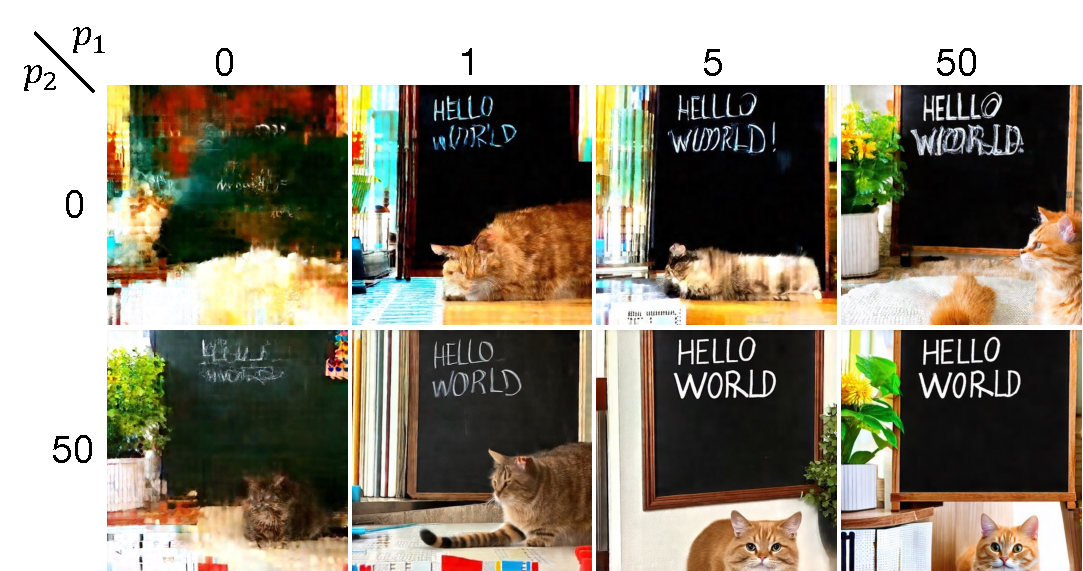
\includegraphics[width=0.8\linewidth]{fig/tradeoff.pdf}
\caption{Image quality-latency tradeoff according to the hyperparameter. Input prompt: ``hello world'' written on the blackboard and a cat.}
\label{fig:tradeoff}
\end{figure}
% Image quality improves toward the bottom-right, accompanied by a corresponding increase in computation latency. 

\niparagraph{Hyperparameter determination algorithm.}
%
Inspired by these insights, we design an offline hyperparameter determination algorithm.
%
% Algorithm~\ref{alg:selection} shows the procedure. 
\sysname sweeps through possible $p_1$ and $p_2$ candidates, generating 64 images for each parameter configuration. 
%
Then, the algorithm determines $p_1$ and $p_2$ by jointly considering (1) the quality of the generated images (measured by FID), and (2) the latency in the hardware.
%
More specifically, we select ($p_1$, $p_2$) with minimum $FID\times latency^{\alpha}$. 
%
While we empirically set $\alpha$ to 0.15 by default, it can be adjusted to prioritize quality or latency.
%
A higher $\alpha$ emphasizes shorter latency, while a lower $\alpha$ prioritizes higher quality. 
% 우리는 이를 위한 offline hyperparameter selection algorithm 을 디자인하였다. 
% 가능한 p_1, p_2 candidates 를 sweep 하면서 적절한 parameter 를 찾는데, 각 parameter configuration 별로 image 를 64개 생성한다. 
% 생성한 이미지의 quality (FID) 와 해당 configuration 에서의 latency 를 동시에 고려하여, optimal p_1, p_2 를 찾는다. 

% \begin{algorithm}[t]
% \footnotesize
% \caption{Hyperparameter Selection Algorithm}\label{alg:selection}
% \begin{algorithmic}[1]
% \renewcommand{\algorithmicrequire}{\textbf{Parameter:}}
% \renewcommand{\algorithmicensure}{\textbf{Output:}}
% \Require $p_1\_{candidates}=[0, 1, 5, 10, 20, 50]$ 
% \Require $p_2\_{candidates}=[0, 10, 20, 50]$ 
% \Ensure $selected\_p_1$, $selected\_p_2$
% \State $selected\_p_1 \gets 0$
% \State $selected\_p_2 \gets 0$
% \State $min\_cost \gets \infty$
% \For{$p_1$ in $p_1\_candidates$}
%     \For{$p_2$ in $p_2\_candidates$}
%         \State $images \gets \text{generate}(p_1, p_2)$ \Comment{generate 64 images}
%         \State $fid \gets \text{calculate\_FID}(images)$
%         \State $latency \gets \text{get\_latency}(p_1, p_2)$ \Comment{get pre-computed latency}
%         \State $cost \gets fid \times latency^\alpha$ \Comment{$\alpha$ is set to 0.15}
%         \If{$cost < min\_cost$} 
%             \State $selected\_p_1, selected\_p_2 = p_1, p_2$
%             \State $min\_cost = cost$
%         \EndIf
%     \EndFor
% \EndFor
% \end{algorithmic}
% \end{algorithm}

\vspace{-0.4cm}
\subsection{\sysname Accelerator Architecture}
\vspace{-0.1cm}
%
\niparagraph{Architecture for precision-flexible MX quantization support.}
%
Figure~\ref{fig:hardware} presents an overview of \sysname architecture.
%
The accelerator is centered around systolic arrays, which are attached with a reordering controller and an MX converter.
%
Systolic arrays perform computations by fetching the input and weight matrices, pre-ordered in MX format, from off-chip memory.
%
After the computation, the reordering controller selects the appropriate output matrix channels from each bank of the output buffer. 
%
For the reordering, the controller maintains a table that specifies the required channel order for each layer and timestep.
%
It forwards these channels in the required order to MX converter.
%
The MX converter then groups and converts the reordered matrix into MX format before storing it in off-chip memory. 
% 
The MX converter is composed of combinational logic, resulting in negligible latency.
% 
The accelerator components operate in a pipelined manner, and the latencies of reordering controller and MX converter are effectively hidden by the significantly larger latency of the systolic array.
% 우리 하드웨어는 systolic arrays, reordering, controller, mx converter 로 이루어져 있다. 
% dataflow 는 다음과 같다. 첫 번째로, off-chip memory 에서 input matrix 와 weight matrix 를 읽어온다. 
% 이 때 off-chip memory 의 weight matrix 및 activation matrix 는 이미 reordered 되어 MX format 으로 저장되어 있다. 
% systolic array 에서 연산을 마치고 나면, reordering controller 가 output buffer 의 각 bank 에 있는 각 channel 들을 적절한 순서로 MX converter 에 보낸다. 
% reordering controller 는 각 layer 및 각 timestep 에서 channel 순서가 어떤 순서로 되어 있어야 하는지를 table 로 가지고 있다. 그 정보를 가지고 reordering 한다. 
% 다음 layer 의 순서로 reordered 된 matrix 가 MX converter 에 의하여 grouping 및 MX format 으로 convert 된 후, off-chip memory 에 저장된다. 

\niparagraph{MX systolic array.}
Our mixed precision technique handles MX6$\times$MX9 (for linear layers), MX9$\times$MX9 (for attention layers), and MX6$\times$MX6 operations. 
The processing elements in the systolic array should support these three types of multiplication. 
We adopted precision-flexible processing element for MX operations proposed in DaCapo~\cite{dacapo}. 
This PE has four 4-bit multipliers that can do the dot product of the 4-bit mantissa.
Therefore, when the group size is 16, MX6$\times$MX6, which needs 4-bit mantissa multiplication, takes 4 cycles per group dot product.
MX6$\times$MX9 and MX9$\times$MX9 need 8-bit mantissa multiplication.
The outputs of the four 4-bit multipliers mentioned above become one 8-bit multiplier output.
Therefore, it takes 16 cycles per group dot product.

% 우리의 mixed precision technique 은 MX6*MX6, MX6*MX9(linear layer), MX9*MX9(attention layer) 연산을 다루고 있다. 
% systolic array 의 processing element 들은 세 종류의 multiplication 을 다룰 수 있어야 한다. 
% MX 를 위한 precision-flexible processing unit 은 Dacapo 에서 제안한 것이 있다. 

% 이 PE 는, 4-bit mantissa 의 dot product 를 할 수 있는 4-bit multiplier 4개를 가지고 있습니다. 
% 따라서 group size 가 16 일 때, MX6 by MX6 는 하나의 group dot product 당 4 cycle이 걸립니다. 
% MX6 by MX9 및 MX9 by MX9 는, 8-bit multiplier 를 사용해야 합니다. 
% 앞서 언급한 4-bit multiplier 4개의 output 이 하나의 8-bit multiplier output 이 됩니다. 
% 따라서, 하나의 group dot product 당 16 cycle 이 걸립니다. 


% Figure
\begin{figure}[t]
\centering
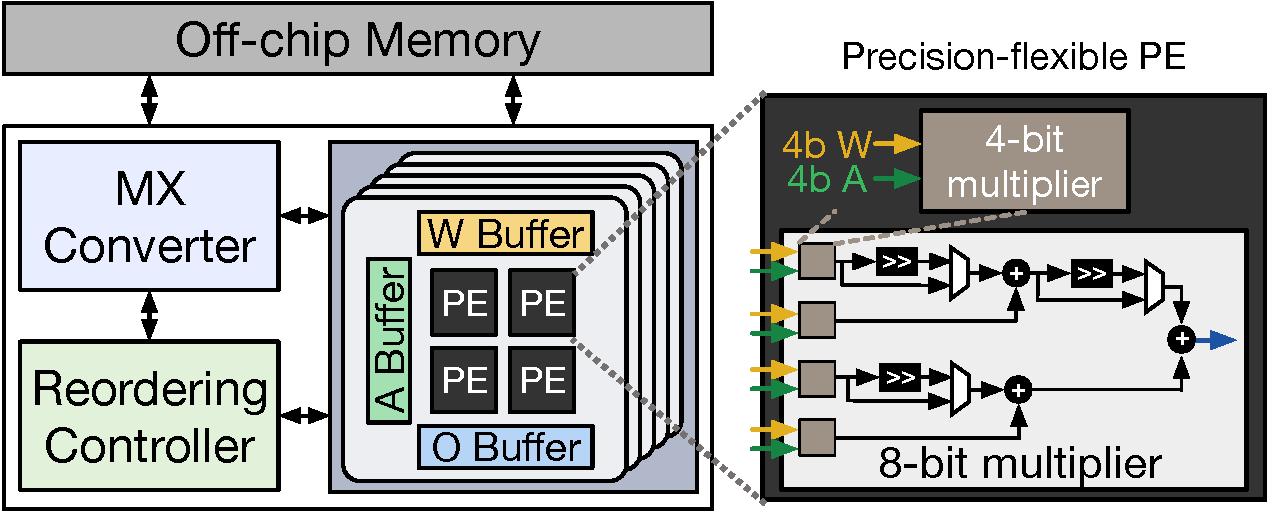
\includegraphics[width=0.85\linewidth]{fig/hardware-cal.pdf}
\caption{\sysname accelerator architecture, built around a systolic array with an MX converter and reordering controller for precision-flexible MX processing.}
\label{fig:hardware}
\end{figure}